%%%%%%%%%%%%%%%%%%%%%%%%%%%%%%%%%%%%%%%%%
% a0poster Landscape Poster
% LaTeX Template
% Version 1.0 (22/06/13)
%
% The a0poster class was created by:
% Gerlinde Kettl and Matthias Weiser (tex@kettl.de)
%
% This template has been downloaded from:
% http://www.LaTeXTemplates.com
%
% License:
% CC BY-NC-SA 3.0 (http://creativecommons.org/licenses/by-nc-sa/3.0/)
%
%%%%%%%%%%%%%%%%%%%%%%%%%%%%%%%%%%%%%%%%%

%----------------------------------------------------------------------------------------
%	PACKAGES AND OTHER DOCUMENT CONFIGURATIONS
%----------------------------------------------------------------------------------------

\documentclass[a0,landscape]{a0poster}

\usepackage{multicol} % This is so we can have multiple columns of text side-by-side
\columnsep=80pt % This is the amount of white space between the columns in the poster
\columnseprule=1pt % This is the thickness of the black line between the columns in the poster

\usepackage[svgnames]{xcolor} % Specify colors by their 'svgnames', for a full list of all colors available see here: http://www.latextemplates.com/svgnames-colors

\usepackage{times} % Use the times font
%\usepackage{palatino} % Uncomment to use the Palatino font

\usepackage{graphicx} % Required for including images
\graphicspath{{figures/}} % Location of the graphics files
\usepackage{booktabs} % Top and bottom rules for table
\usepackage[font=small,labelfont=bf]{caption} % Required for specifying captions to tables and figures
\usepackage{amsfonts, amsmath, amsthm, amssymb} % For math fonts, symbols and environments

\usepackage{wrapfig} % Allows wrapping text around tables and figures



\usepackage[utf8]{inputenc} % Pour utiliser les caractères accentués
\usepackage{tikz}
\usetikzlibrary{shapes,snakes}
\usetikzlibrary{positioning}
\usepackage[export]{adjustbox}
\usepackage[skins,listings,breakable,listingsutf8,theorems,hooks,fitting]{tcolorbox}
\usepackage[round]{natbib}
\tcbuselibrary{raster}
\begin{document}

%----------------------------------------------------------------------------------------
%	POSTER HEADER
%----------------------------------------------------------------------------------------

% The header is divided into three boxes:
% The first is 55% wide and houses the title, subtitle, names and university/organization
% The second is 25% wide and houses contact information
% The third is 19% wide and houses a logo for your university/organization or a photo of you
% The widths of these boxes can be easily edited to accommodate your content as you see fit

\noindent\begin{minipage}[b]{\linewidth}
\centering
\noindent \veryHuge \color{NavyBlue} \textbf{Projected changes to hydrometeorologic extremes across Canada} \color{Black}\\ % Title
\noindent\begin{minipage}[c]{0.2\linewidth}
      \center
      
\includegraphics[width=25cm]{logo_cnrcwp_escer.png} % Logo or a photo of you, adjust its dimensions here
\end{minipage} \hfill
%
\begin{minipage}[c]{0.15\linewidth}
  \center
  \Large \textbf{Oleksandr Huziy} \\
  \large \texttt{guziy.sasha@gmail.com}
\end{minipage}
%
\begin{minipage}[b]{0.01\linewidth}
 \center
 \Large\&
\end{minipage}
%
\begin{minipage}[c]{0.15\linewidth}
   \center
   \Large \textbf{Dae Il Jeong} \\
   \large  \texttt{dae.jeong2@gmail.com}
\end{minipage}\hfill
%
\begin{minipage}[b]{0.01\linewidth}
 \center
 \Large\&
\end{minipage}
%
\begin{minipage}[c]{0.15\linewidth}
   \center
   \Large \textbf{Laxmi Sushama} \\
   \large  \texttt{sushama.laxmi@uqam.ca}
\end{minipage}\hfill
%
\begin{minipage}[c]{0.2\linewidth}
  \center
  
\includegraphics[width=15cm]{logo_uqam.png} % Logo or a photo of you, adjust its dimensions here
\end{minipage}
\rule{\linewidth}{3pt}
\end{minipage}
%

\vspace{0.5cm} % A bit of extra whitespace between the header and poster content

%----------------------------------------------------------------------------------------

\begin{multicols*}{4} % This is how many columns your poster will be broken into, a poster with many figures may benefit from less columns whereas a text-heavy poster benefits from more

%----------------------------------------------------------------------------------------
%	INTRODUCTION
%----------------------------------------------------------------------------------------

\color{DarkSlateGray} % SaddleBrown color for the introduction

\section*{(A) Introduction}
The Fifth Assessment Report of the Intergovernmental Panel on Climate Change
concluded that there will be an intensification of the hydrological cycle in the
future warmer climate. It was also reported that the frequency and intensity of
extreme precipitation events have likely increased over North America and Europe
since around 1950 \citep{hartmann2013} and that it will very likely increase
over most mid-latitude land-masses in future climate \citep{collins2013}.

In this study the changes in hydro-meteorological extremes are assessed over
Canada, using transient climate change simulations of the fifth generation of
Canadian Regional Climate (CRCM5) model. Specifically, the results are reported
on changes to the rain on snow events over North America, heat wave events over
Canada, high and low flow streamflow values \citep{huziy2016impact} both using
univariate and multivariate analysis over northeastern Canadian watersheds.



%----------------------------------------------------------------------------------------
%	OBJECTIVES
%----------------------------------------------------------------------------------------

\color{DarkSlateGray} % DarkSlateGray color for the rest of the content

\section*{(B) Main Objectives}
\begin{tcolorbox}[colback=white,colframe=green!40!black]
  \color{DarkSlateGray}
  \begin{enumerate}
    \item Summarize our recent results on projected changes to characteristics of hydrometeorologic extremes.
    \item Analyze links and coherency of the results from different experiment configurations.
  \end{enumerate}
\end{tcolorbox}

%----------------------------------------------------------------------------------------
%	MATERIALS AND METHODS
%----------------------------------------------------------------------------------------

\section*{(C) Methods and experiment configurations}
\subsection*{C.1 Methods}
%
\begin{itemize}
  \item how rain on snow days determined
  \item how heat wave days are determined
  \item how return levels are calculated
  \item How copula is used
\end{itemize}

\subsection*{C.2 Experiment setup}

\begin{tcolorbox}[colback=white,colframe=green!40!black]
\center
\begin{tabular}{c|c|c|c|l}
    Section & $\Delta x$ & Current period & Future Period & Additional information \\
    \hline\hline
    D.1    & 0.1$^\circ$ & 1980-2010      & 2070-2100     & \begin{minipage}{8cm}\flushleft lakes: Hostetler, rivers: WATROUTE-modified \end{minipage}\\
    D.2    &             & \\
    D.3    &             &\\
    D.4    &             &\\
    \hline
\end{tabular}

\vspace{2cm}
\begin{minipage}{\linewidth}
 *Atmosphere is modelled using various CRCM configurations in all presented experiments.
\end{minipage}
\end{tcolorbox}

\vfill

%----------------------------------------------------------------------------------------
%	RESULTS
%----------------------------------------------------------------------------------------

\section*{(D) Results}

\subsection*{D.1 Rain on snow events over North America}
\begin{minipage}[t]{\linewidth}
\begingroup
\setlength{\columnsep}{30pt}
\begin{wrapfigure}{l}{0.6\linewidth}
  \center
  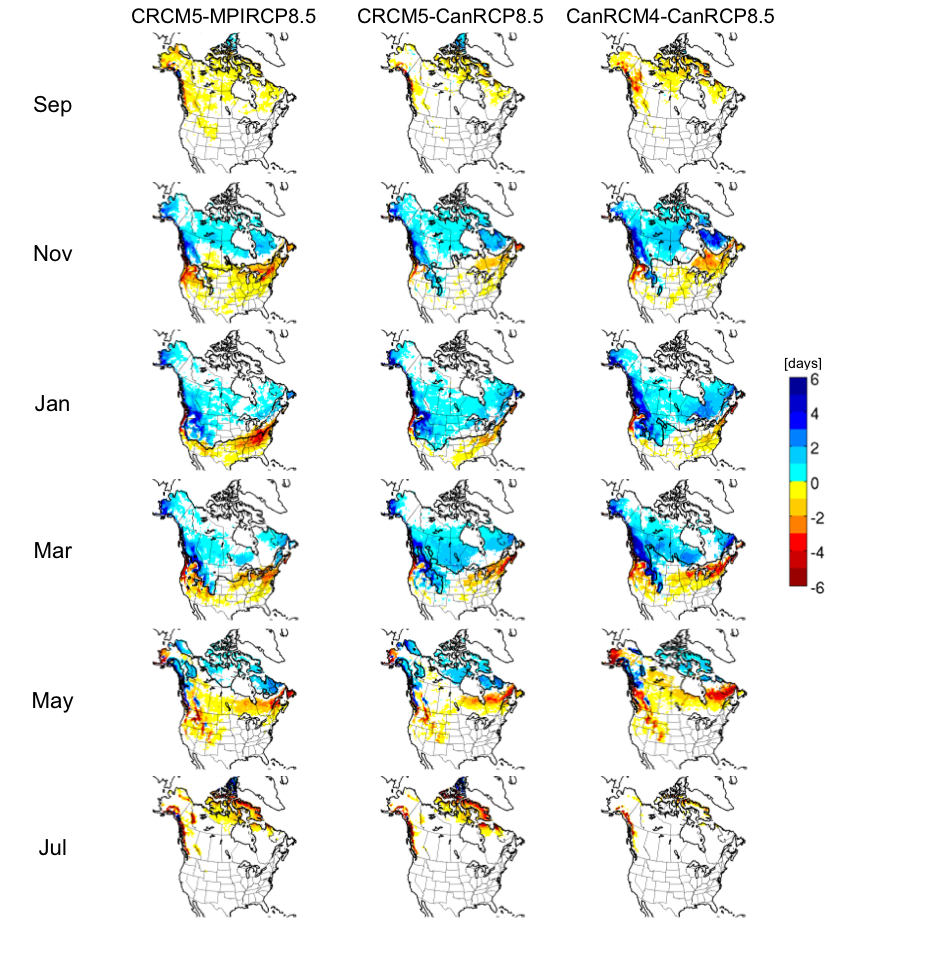
\includegraphics{cc_num_of_ros}
  \captionof{figure}{\label{fig_cc_num_of_ros}\color{Green} Projected changes to the number of ROS days for the three RCM simulations (i.e.,
                                  CRCM5-MPIRCP8.5, CRCM5-CanRCP8.5, and CanRCM4-CanRCP8.5) for the future
                                  2041-2070 period with respect to the current1976-2005 period. The black contour
                                  represents the mean freezing line in future climate. Projected changes are shown
                                  when they are statistically significant with the two-sample t-test at the 10\%
                                  significance level.
                                  }
\end{wrapfigure}
Figure \ref{fig_cc_num_of_ros} shows
projected changes to monthly number of rain on snow (ROS) days, for CRCM5-MPIRCP8.5, CRCM5-CanRCP8.5, and CanRCM4-CanRCP8.5. The three
simulations generally show increases in the future ROS characteristics to the
north of the future freezing line, particularly from November to May. (Sasha
added, please, check) The decreases at the start and end of the cold season are
due to the shortening of the cold season and the increases in the middle of
winter are caused by the increased fraction of liquid precipitation during
colder periods.

\endgroup
\end{minipage}
\vspace{2cm}


\subsection*{D.2 Heat wave events over Canada}
\begin{minipage}[t]{\linewidth}
  \begingroup
  \setlength{\columnsep}{30pt}
  \begin{wrapfigure}{r}{0.6\linewidth}
  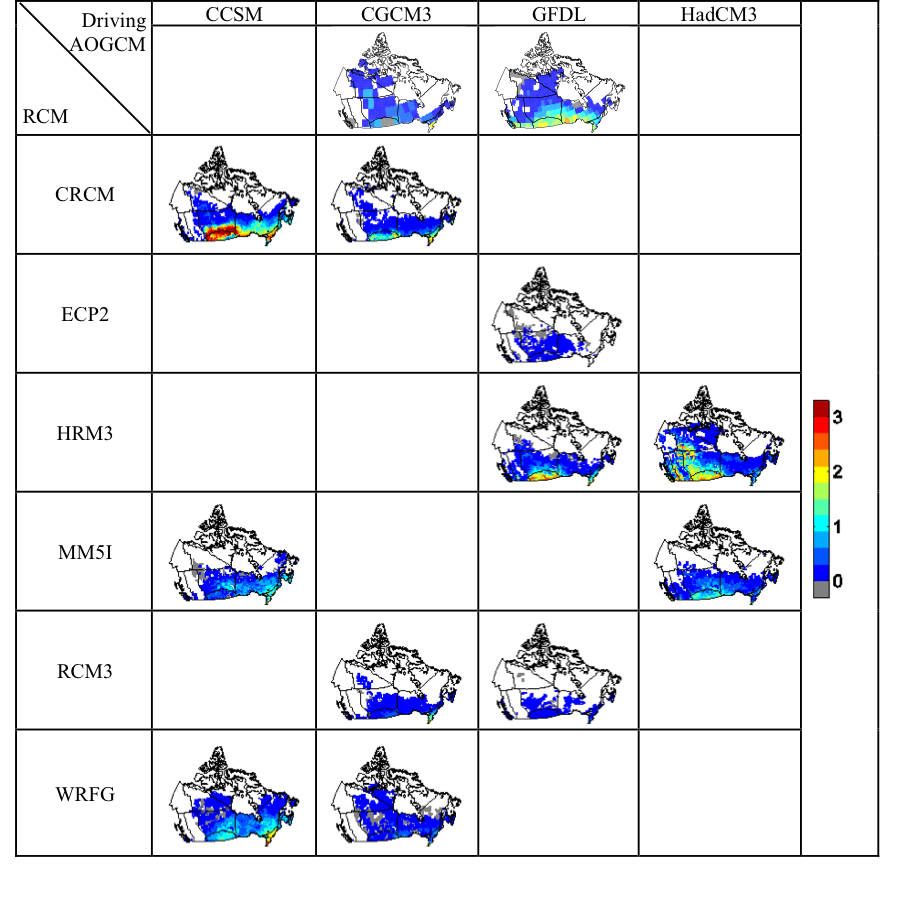
\includegraphics[width=\linewidth]{cc_heatwaves}
  \captionof{figure}{\label{fig_cc_heatwaves}\color{Green} Projected changes to the number of heat wave events per summer for the 2 driving
                                  AOGCMs and 11 RCM-AOGCMs for the future 2040–2069 period with respect to the
                                  current 1970–1999 period. Grid points are colorless if simulations do not yield
                                  any heat wave event for both periods.
                                  }
  \end{wrapfigure}
  Projected changes to the number of heat wave events for the future period with
  respect to the current period of 11 RCM-AOGCMs and 2 driving AOGCMs are shown in
  Fig. \ref{fig_cc_heatwaves}. These changes are robust as all the 11 RCM-AOGCMs and 2 AOGCMs generally
  show an increase in the number of heat wave events for southern Canada, where
  the 90\textsuperscript{th} percentile of Tmax is near 32${^\circ}$C, i.e., the threshold of heat wave, for
  the 1981–2003 summer period, compared to other regions.

  \endgroup
\end{minipage}
\vfill





% \begin{tcbitemize}[raster columns=2, raster equal height]
%
% %\tcbitem[colback=white,colframe=white,sidebyside align=top,sidebyside]
%   \tcbitem[colback=white,colframe=green!40!black, adjusted title={Lake-atm. interactions (Fig. \ref{fig_la_and_lr}a)}]
%   \color{DarkSlateGray}
%   \begin{itemize}
%     \item Impact of lake-atm. interactions is mostly positive, but modest.
%   \end{itemize}
%
% \tcbitem[colback=white,colframe=green!40!black, adjusted title={Lake-river interactions (Fig. \ref{fig_la_and_lr}b)}]
%   \color{DarkSlateGray}
%   \begin{itemize}
%     \item Winter impacts are positive and significant for the bigger northern part of the domain due to additional water coming to the river network from lakes.
%     \item Mostly negative impacts are obtained in spring since part of water from snow melt is stored in lakes to be released later into the river network.
%   \end{itemize}
%
% \end{tcbitemize}



\subsection*{D.3 Projected changes to high and low flow return levels for major Quebec watersheds}
\begin{minipage}[t]{\linewidth}
  \begin{minipage}[t]{0.5\linewidth}
      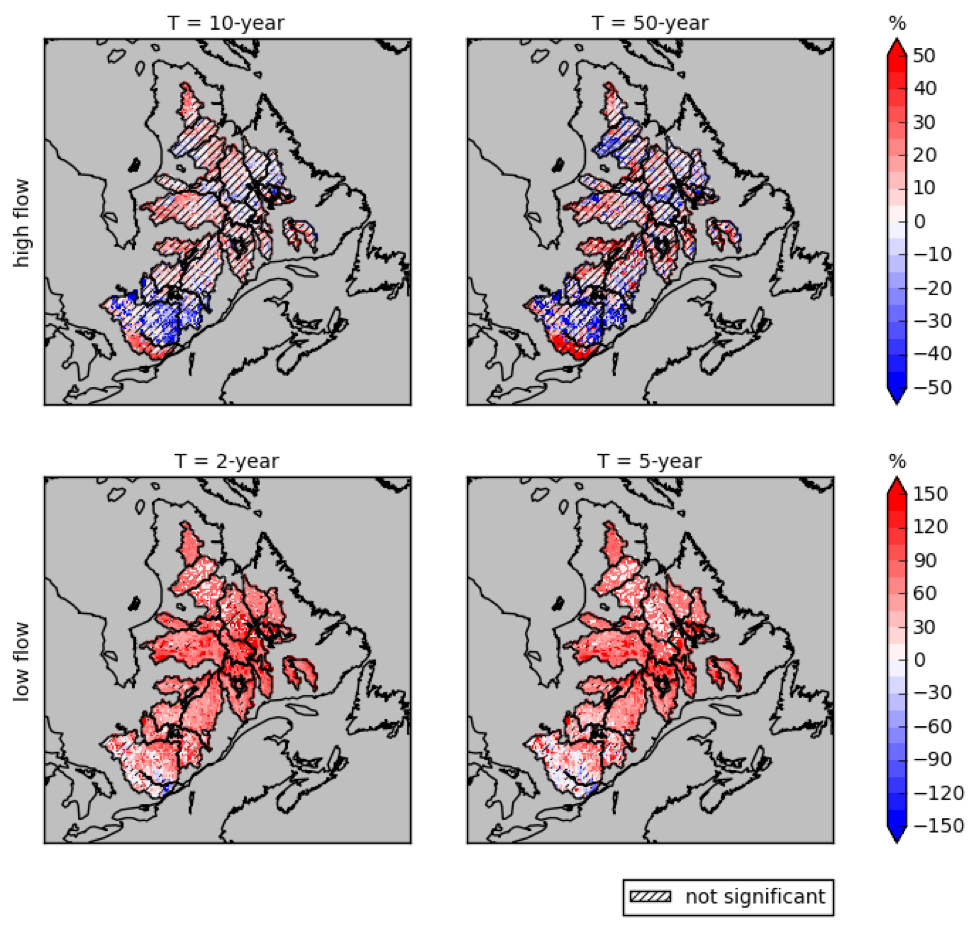
\includegraphics[width=0.95\linewidth]{extreme_low_and_high_flow_RL}
      \captionof{figure}{\color{Green}
      Projected changes for the 2070–2100 period with respect to the 1980-2010 period
      to the 10- and 50-year return levels of 1-day high flow (upper panel) and of 2-
      and 5-year return levels of 15-day low flow (bottom panel) for CanESM2-CRCM5-L.
      Changes that are not significant at the 5\% significance level (evaluated using
      bootstrap procedure) are hatched over.
      }
  \end{minipage}
  \hfill
  \begin{minipage}[c]{0.45\linewidth}
    \center
    \begin{itemize}
      \item Almost no significant changes to high flow return levels are detected for future climate.
      \item The changes to the low flow return levels are mostly positive and significant at the 5\% significance level over all studied watersheds.
      \item Some decreases to the low flow return levels are noted in the southern part of the domain, which might indicate reduced groundwater contribution to streamflows during low flow periods at those points in future climate due to enhanced summer evaporation and reduced summer and fall precipitation.
      \item For more details see \citet{huziy2016impact}.
    \end{itemize}
  \end{minipage}
\end{minipage}



\subsection*{D.4 Extreme flow characteristics for Quebec watersheds based on a multivariate distribution}
%
\begin{minipage}[t]{\linewidth}

\begingroup
  \setlength{\columnsep}{30pt}

  \begin{wrapfigure}{r}{0.6\linewidth}
    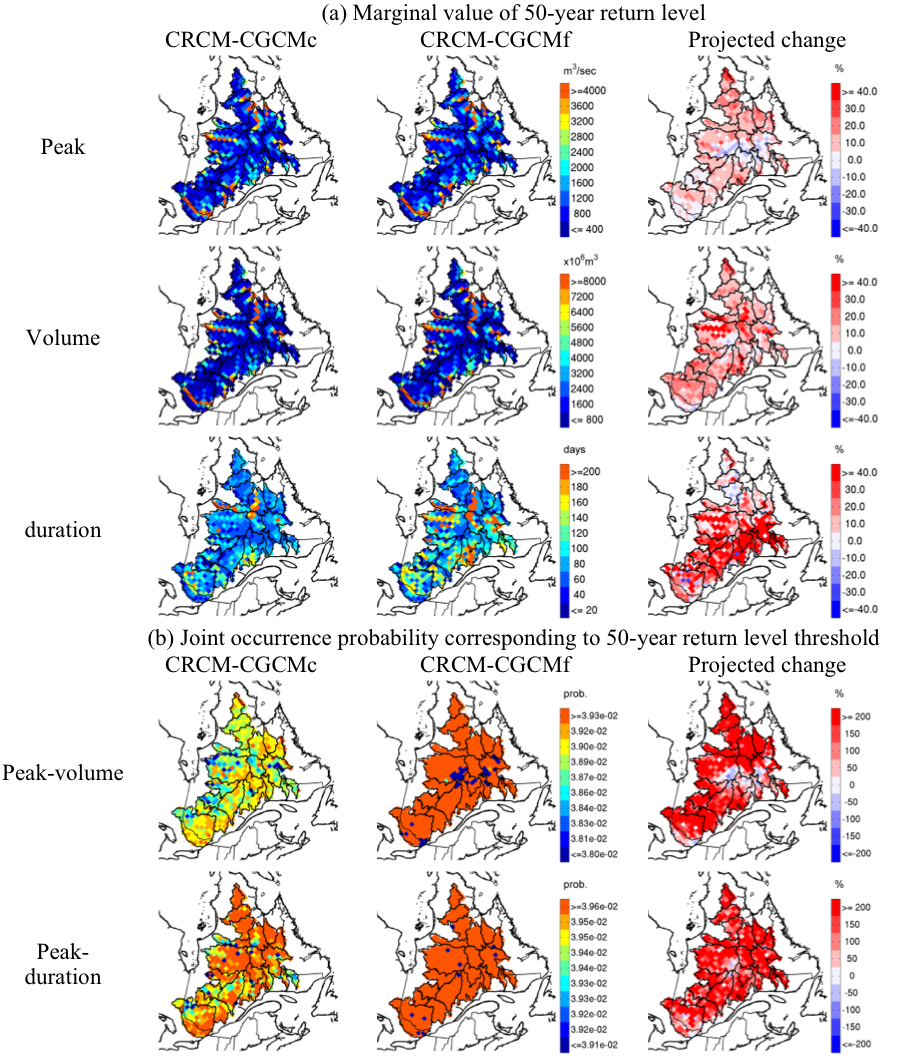
\includegraphics[width=\linewidth]{cc_copula}
    \captionof{figure}{\label{fig_cc_copula}\color{Green} Fifty-year return levels of (a) peak, volume and duration and their joint
                occurrence probabilities computed using merged longer samples for CRCM-CGCMc
                (column 1) and CRCM-CGCMf (column 2). Percentage difference between CRCM-CGCMf
                and CRCM-CGCMc is shown in column 3.}
  \end{wrapfigure}
  Fig. \ref{fig_cc_copula} presents marginal return values and joint occurrence probabilities for
  50-year return period for CRCM-CGCMc and CRCM-CGCMf, estimated using merged
  series. Percentage changes in marginal return levels and P1 and P2 values are
  also shown. On average, the projected changes to marginal 50-year return levels
  of flood peak, volume and duration suggest increases in future climate. The
  projected increases in the flood peak, volume and duration for the majority of
  the basins are caused by increased winter and spring precipitation and warmer
  spring temperatures, leading to increased spring snowmelt in future climate.
  Projected changes to the joint occurrence probabilities of the peak-volume,
  peak-duration and volume-duration pairs of flood characteristics were studied
  for the very first time for the 21 watersheds considered in this study. Results
  suggest future increases for the joint occurrence probabilities with larger
  increases for longer return periods than shorter return periods.

\endgroup
%
\end{minipage}
\hfill
\vspace{2cm}



%----------------------------------------------------------------------------------------
%	CONCLUSIONS
%----------------------------------------------------------------------------------------

\color{SaddleBrown} % SaddleBrown color for the conclusions to make them stand out

\section*{(E) Conclusions}

\begin{itemize}
\item D.1 and D.3: Increased low flow values in D.3 agree with
the shortening of the cold period and increased fraction of liquid precipitation
projected in D.1.

\item D.2 and D.3: Increased number of heat wave in D.2 is
in-line with the decreasing low flow amplitudes in the southern part of the
domain.

\item Simulations over bigger regions and the complete analysis of both
atmospheric fields and streamflows are required to further improve our
confidence in the relationships between projected changes to the parameters of
hydrometeorologic extremes.
\end{itemize}

\color{DarkSlateGray} % Set the color back to DarkSlateGray for the rest of the content


 %----------------------------------------------------------------------------------------
%	REFERENCES
%----------------------------------------------------------------------------------------

\nocite{*} % Print all references regardless of whether they were cited in the poster or not
\small
\bibliographystyle{agu} % Plain referencing style
\bibliography{sample} % Use the example bibliography file sample.bib

%----------------------------------------------------------------------------------------
%	ACKNOWLEDGEMENTS
%----------------------------------------------------------------------------------------
\section*{Acknowledgements}
\small
This research was carried out within the Canadian Network for Regional Climate and Weather Processes (CNRCWP) project funded by the Natural Sciences and Engineering Research Council (NSERC) of Canada.
%----------------------------------------------------------------------------------------

\end{multicols*}
\end{document}
